\chapter{Preparação dos dados}
\label{ch:preparacao}

Na etapa de preparação dos dados, a representação da rede propriamente dita é
mensurada. Apesar dessa mensuração ser por si só um processo de mineração de
dados, apresentamos como pertencente à etapa de preparação porque o intento final
é a análise de influência que vai ser feita em cima da rede, não a rede em si.
Neste capítulo, portanto, apresentaremos algumas técnicas de mineração de dados
para a mensuração da rede, as dificuldades existentes quando se utiliza
aprendizagem de máquina e faremos algumas considerações sobre técnicas para a
escolha dos dados mais relevantes.

Trataremos aqui principalmente de mensurações da rede, que é a primeira parte do
processo de análise de influência. A mensuração, por sua vez, se divide em dois
momentos: dados \textbf{brutos} e dados \textbf{compilados}. No seu estado bruto,
a rede guarda os dados como se lhe apresentam através dos medianeiros, por
exemplo: quantidade de interações, tamanho das interações, classificações usadas,
data da interação, etc. Esse processo por si so é trabalhoso, pois devemos ter o
cuidado de guardar não só as interações, mas as propriedades relacionadas a elas.
Também é comum a formação de hipergrafos, isto é, grafos onde os atores são
agrupados por alguma relação \citep{Breiger1974, Seidman1978}. Um exemplo
claro de hipergrafo é a representação formada a partir da afiliação dos atores à
comunidades, contudo, a rigor, toda interação particiona o grafo em um
subconjunto.

\section{Exemplo de hipergrafo}

Considere dois medianeiros $A$ e $B$ que mediam o mesmo conjunto de
atores $\mathscr{N} = \{n_1, n_2, n_3\}$. Em $A$, coletamos duas interações
$i_1$ e $i_2$. O ator $n_1$ é o autor de ambas interações. O ator $n_2$ é o
receptor da interação $i_1$ e o ator $n_3$ é o receptor da interação $i_2$. Se
construirmos uma matriz de adjacência e um hipergrafo a partir do medianeiro $A$
teremos o resultado apresentado na \figref{fig:hiperg1}:

\begin{figure}[htb]
  \centering
  \begin{minipage}[c]{0.48\textwidth}
    \centering
    \begin{array}{c | c c c}
	& n_1 & n_2 & n_3 \\ \hline
	n_1&0&1&1\\
	n_2&0&0&0\\
	n_3&0&0&0\\
	\end{array}
  \end{minipage}
  \begin{minipage}[c]{0.38\textwidth}
    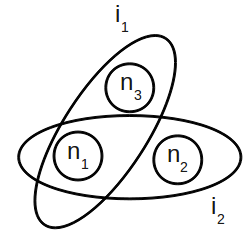
\includegraphics[width=\textwidth]{imgs/hipergraf1v.png}
  \end{minipage}
  \caption{hipergrafo de $A$ -- três atores, duas
  interações.}\label{fig:hiperg1}
\end{figure}

Já em $B$ temos apenas uma interação, $i_3$, cujos receptores são $n_2$ e $n_3$.
Se construirmos sua matriz de adjacência, ela será igual à de $A$ porem os
hipergrafos demonstram grande diferença, já que em $B$ o ator $n_1$ alcançou
$n_2$ e $n_3$ com uma única interação.

\begin{figure}[htb]
  \centering
  \begin{minipage}[c]{0.48\textwidth}
    \centering
    \begin{array}{c | c c c}
	& n_1 & n_2 & n_3 \\ \hline
	n_1&0&1&1\\
	n_2&0&0&0\\
	n_3&0&0&0\\
	\end{array}
  \end{minipage}
  \begin{minipage}[c]{0.28\textwidth}
    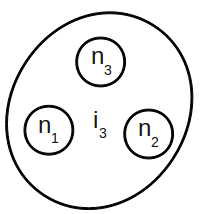
\includegraphics[width=\textwidth]{imgs/hipergraf2v.png}
  \end{minipage}
  \caption{hipergrafo de $B$ -- três atores, uma
  interação.}\label{fig:hiperg2}
\end{figure}

Nenhum das abordagens citadas no \chapref{ch:dominio} consideram o aspecto de
hipergrafo das interações. Seria necessário adaptar as técnicas de análise de
influência se quisermos considerar um ator que influencia muitos em uma única
interação de outro que o faz através de muitas interações separadas. Tendo isso
em mente, partimos para as técnicas de mensuração em si.

\section{Interações não-textuais}

Uma possível abordagem foi a citada no exemplo acima, a da ausência ou presença
de interação. Ela foi usada por \citet{Xiang2010} e simplifica a representação
em uma rede dicotômica. Outras possibilidades está em contar a quantidade de
interações ocorridas, a frequência por período, a idade da primeira interação, a
presença em comunidades comuns, similaridade de perfil, etc. De forma geral
podemos criar a rede por:

\begin{itemize}
\item Intensidade/Quantidade
\item Frequência
\item Presença/Ausência
\item Properidade única (e.g., Longevidade)
\item Similaridade
\end{itemize}

Cada uma dessas apresenta apenas uma dimensão da relação, de forma que para o
mesmo medianeiro mais de uma representação pode ser mensurada a partir de
diferentes formas de agregação. Outras representações ainda podem ser criadas a
partir da combinação de mensurações diferentes, por exemplo: intensidade x
frequência, longevidade x similaridade. Deve-se ter um cuidado extra no uso de
agregações porque podem introduzir correlações espúrias no conjunto de dados,
levando a erros do tipo I (falso positivo) e tipo II (falso negativo), pois a
agregação mascara quais elementos estão correlacionados de fato
\citep{Jensen2003}. Não existe forma correta de escolher as agregações, porém
veremos mais adiante como poderemos diminuir o impacto disso no processo como um
todo.

No final, teremos uma ou mais representações da rede para cada tipo de
medianeiro, que por diferença de natureza não são facilmente integráveis.
Contando, porém, com uma análise intrínseca dos medianeiros, poríamos apostar
numa integração pela teoria da atenção. Apesar de que tempo gasto não se traduz
diretamente em atenção dispendida, poderíamos mensurar o tempo que o usuário do
medianeiro empregou em cada interação e daí inferir uma valor em unidade única:
atenção \citep{Davenport2001}. Com isso teríamos o tempo empregado na
visualização de um vídeo, de uma foto como estimativa da atenção. Essa análise
nem sempre é possível e mesmo que seja, há interações que são naturalmente
difíceis de integrar, como as avaliações (\emph{ratings}, \emph{rankings}). As
avaliações tomam sempre o mesmo tempo (o do clique do mouse) e seu conteúdo é
totalmente ``emocional'', isto é, polarizado entre positivo e negativo. Caso seja
utilizado técnicas de análise de sentimentos para as outras interações, então
talvez as avaliações possam ser integradas pela dimensão emocional da força da
relação. Por outro lado, avaliações são excelentes opções para a utilização como
grupo de teste para algoritmos de aprendizagem de máquina ``supervisionados''.

\section{Interações textuais}

Na seção anterior investigamos as relações não-textuais, agora vamos nos deter
nas textuais. Primeiramente, intentamos com essa divisão alcançar uma
consequência prática: a integração de diversas interações numa só rede. A rede
que vamos construir é valorada, isto é, as conexões possuem um peso na forma de
um número real dentro de um intervalo. Ao contrário de redes binárias, as redes
valoradas proporcionam um indicativo da \textbf{força} da conexão entre os
atores.

Dentro de uma teoria da atenção como capital social, devemos então nos voltar
para a afirmação de que laços por onde trafegam muitos recursos são laços fortes
e o contrário também é verdade. Em cada interação na rede, como vimos, tem um
ator-agente que inicia a interação e um grupo de abrangência, que chamaremos de
atores-receptores, que é afetado por ela. Com esse modelo, podemos estimar que
os receptores cedem atenção para o agente e a recíproca também é verdadeira,
pois o agente escolheu interagir com este grupo e essa escolha já é um
indicativo de atenção cedida.

Idealmente, essa atenção poderia ser mensurada a partir do tempo empregado pelos
atores na interação, mas quase nunca essa informação está disponível. Por esta
razão, sugerimos a quantidade de palavras na interação textual como uma
estimativa para a quantidade de atenção trocada na interação. A sugestão advém
naturalmente do fato de que quanto maior o texto, mais tempo é empregado na sua
leitura, possivelmente mais recursos cognitivos também serão empregados para a
sua apreensão. Isso nem sempre é verdade para todos os textos, ou tipos de
textos, mas restringindo nosso escopo para comunidades virtuais de amigos e/ou
comunidades de prática \citep{Lave1991, Lave1991a}, acreditamos ser esse
um bom ponto de partida.

Outro cuidado necessário é na determinação se de fato a interação foi percebida
pelos receptores. Na maioria das vezes essa determinação é inviável, aumentando
a incerteza do modelo. Entretanto, um recurso simples que pode ser utilizado é
procurar por interações encadeadas, isto é, quando uma interação posterior é 
reação a outra anterior. Por exemplo, quando uma mensagem é respondida, um texto
é comentado, um conteúdo é recomendado, em todos esses casos podemos avaliar que
o agente que reagiu não só percebeu a interação do agente anterior, como se deu
o trabalho de responder. Em verdade, para interações que normalmente se
encadeiam como \emph{threads} de fórums ou listas de discussão, podemos
considerar a resposta como um sinal de atenção não só para com o participante
imediatamente anterior, mas para vários antes dele que de certa forma
influenciaram na resposta atual.

Assim, podemos construir uma rede onde os nós são os atores e os laços é o
somatório da atenção trocada pelos mesmos. Quanto mais textos de um ator $a$
lidos, respondidos, recomendados, avaliados por um ator $b$, maior será a força
da relação direcionada de $b$ para $a$. Quanto mais conteúdo um ator $a$ publica
para um determinado público, mais forte também será sua relação direcionada
com o mesmo. Tal rede, por tanto, integraria insumos de diversos tipos de
interação mensurados, desde que sejam de conteúdo textual.

\subsection{Algoritmo}
\label{sec:formalizacao}

Utilizando a teoria da atenção como capital social apresentada na
\secref{sec:teoria_atencao}, construímos um algoritmo simples para mensurar a
rede. A entrada do algoritmo é o conjunto de \textbf{interações textuais}. A
saída é uma matriz de adjacência $X$ entre os atores onde a posição $x_{ij}$
guarda a ``quantidade de atenção'' que o $i$-ésimo ator cede para o $j$-ésimo
ator. A forma geral do algoritmo é a que segue:

\begin{itemize}
  \item para cada interação $l$ no conjunto de interações: \begin{itemize}
    \item para cada receptor de $l$: \begin{itemize}
      \item a atenção total que vai do autor para o receptor é acrescida pelo
      valor da \textbf{atenção residual} de $l$;
      \item a atenção total que vai do receptor para o autor é acrescida pelo valor da
		\textbf{atenção direta} de $l$;
	  \item	para cada mensagem $t$ na \emph{thread}\footnote{\emph{thread} é uma
	  cadeia de mensagens que sucedem-se no tempo pela relação de resposta. A
	  mensagem que inicia a \emph{thread} não é uma resposta a nenhuma outra
	  interação e todas as outras mensagens da \emph{thread} são respostas a alguma outra mensagem
	  também da \emph{thread}, mas que ocorreu antes.} de $l$:
	  \begin{itemize}
	    \item a atenção total que vai do autor de $l$ para o autor de $t$ é
			acrescida pelo valor da \textbf{atenção transitiva} de $l$ para $t$;
		\end{itemize}
	\end{itemize}
\end{itemize}	
\end{itemize}
		 
A atenção direta de uma interação é a sua quantidade de palavras multiplicada
por um \textbf{fator de concentração} que limita a quantidade de atenção cedida
por um receptor que apenas leu a interação para apenas uma fração do que poderia
ter cedido. O fator de concentração é um parâmetro do algoritmo e
serve para diferenciar receptores que apenas receberam a interação
daqueles que responderam a ela. 

A atenção residual de uma interação é a sua quantidade de palavras dividida pela
quantidade de seus receptores. Dessa forma, cada receptor recebe apenas uma
fração da atenção total cedida pelo autor, de modo que quanto mais receptores
uma interação possuir, menos atenção cada receptor recebe individualmente.

A atenção transitiva é o complemento da direta e fortalece as conexões entre os
indivíduos que respondem uns aos outros. Consiste na diferença entre a
quantidade de palavras de uma interação e sua atenção direta, i.e., $(1 -
\text{fator de concentração})$ x quantidade de palavras. A atenção transitiva
pode ainda ser moderada pela distância que as duas interações tem na
\emph{thread}. Assim, o resultado anterior é multiplicado pela \textbf{função de
esquecimento} que tem como o parâmetro a distância entre as interações. A
distância entre as interações é calculada da seguinte forma:

\begin{itemize}
  \item A interação $l$ tem distância 0 para consigo mesma;
  \item Se $l$ é uma resposta a $t$ então a distância entre elas é 1;
  \item Se $l$ é uma resposta a $t$ então a distância entre $l$ e uma interação
  $m$ qualquer é $1 + \text{distância}(t, m)$;
  \item Se $l$ não é uma resposta a nenhuma outra interação, a distância dela
  para qualquer outra interação é infinita.
\end{itemize}

Evidentemente, este é um modelo exploratório para a mensuração de redes a partir
de interações textuais sob um ponto de vista generalista. Nesse sentido há muito
espaço para aperfeiçoamento dentro do campo experimental.

\section{Critérios de escolha da representação}
\label{sec:criterios}
Qual a rede ideal para a análise de influência? Não há resposta objetiva para
essa pergunta. Cada rede é uma representação de um fenômeno social que vai além
das ferramentas, mesmo sendo capaz de coletar e integrar todas as interações
digitais, as pessoas ainda vão ser capazes de tomar café juntas e nossa visão
será apenas parcial. Sendo assim, é evidente que cada representação mensurada é
uma parte da informação e, portanto, capaz de descrever aspectos diferentes ou
não do fenômeno. São essas variações entre as representações de redes que
chamaremos de \textbf{critérios de escolha}.

Para enteder sua utilidade, um exemplo: imaginemos que ao final da análise
tenhamos duas ou mais representações da rede: uma textual e algumas não textuais.
Para cada uma encontramos valores diferentes de proeminência, então qual usar?
Colocando de outra forma, quanto de informação estarei perdendo caso considere
apenas uma delas?

A seleção de característica (\emph{feature selection}), na aprendizagem de
máquina, é a tarefa de escolher quais variáveis -- ou produtos, ou transformações
destas -- serão consideradas no treinamento do sistema de forma a obter a melhor
aproximação do modelo \citep{Jain1997, Blum1997, Jain2000}. De forma similar
devemos ser capazes de selecionar redes que maximizem nossa análise de
influência. Recentemente, \citet{Peng2005} sugere que as variáveis sejam
escolhidas de forma a maximizar a relevância e reduzir a redundância, mRMR
(\emph{minimal-redundancy-maximal-relevance}). No nosso caso, não conhecemos o
modelo da rede \emph{a priori} e a inferência é não-supervisionada. Por isso, não
temos como avaliar a relevância de uma rede em relação a outra, todas são
relevantes. Podemos considerar que redes que não demonstrem características de
redes sociais serão vistas como fortemente enviesadas e por isso de baixa
relevância, a saber: diâmetro pequeno (\emph{small world}) \citep{Milgram1967,
Watts1998}, poucos muito conectados e muitos pouco conectados (\emph{power-law})
\citep{Liljeros2001, Mitzenmacher2004} e atores com muitas conexões tendem a
estar conectados uns aos outros (\emph{scale-free}) \citep{Li2005}.

Por outro lado, a redundância da informação nos ajudará a separar as
representações importantes das que não acrescentam informação substancial, ou
seja, são redundantes. Sendo assim, nosso objetivo é formular alguns critérios
de escolha, de modo que tenhamos em mãos o conjunto de representações
minimamente redundante.

\subsection{Mínima redundância}

Dada uma entrada de dados $D$, composta de $N$ amostras e $M$
características $X=\{x_i, i=1,\ldots,M\}$, dizemos que um subconjunto $S
\subseteq X$ de $m$ características $\{x_i\}$ é mínimamente redundante se atende
a condição:

\begin{equation}
\label{def:min_redun}
\min R(S), R = \frac{1}{|S|^2}\sum_{x_i, x_j \in S}I(x_i;x_j)
\end{equation}

$I(.)$ é a função de informação mútua e que mede uma forma de dependência entre
duas variáveis aleatórias. Dado duas variáveis aleatórias discretas, $X$ e $Y$
definimos a informação mútua de ambas como:

\begin{equation}
\label{def:inf_mutua}
I(X;Y) = \sum_{x\in X}\sum_{y\in Y}p(x,y)\log \frac{p(x,y)}{p(x)p(y)}
\end{equation}

Um dos inconvenientes de utilizar a função de mútua informação como definida é
que no caso de redes sociais, cada conexão pode ser considerada como uma
variável aleatória de resultados possíveis $\{0,1\}$ quando binária, ou um
intervalo definido. Se assim for, não podemos dizer muito da probabilidade da
relação existir ou não (por enquanto). Se por outro lado considerarmos a
variável como sendo a prossibilidade da presença da relação (para simplificar) e
cada par de atores uma amostra dessa variável, então estaremos encontrando
dependência ou correlação sobre a densidade da rede apenas, deixando de lado
importante padrões estruturais como a transitividade e a reciprocidade. Por esta
razão, precisamos adaptar nossa função de mútua informação para considerar as
peculiaridades das redes sociais. 

\subsection{Redundância das conexões}

Uma conexão é redundante quando pode ser encontrada em mais de uma rede. Mais do
que isso, duas redes são redundantes quando além de compartilhar conexões também
compartilham determinados padrões como triângulos e subgrupos. As duas
famílias de ferramentas para acessar essa similaridade estrutural mais
desenvolvidas na literatura são: gráficos aleatórios exponenciais e procedimento
de atribuição quadrática, respectivamente $p*$ (\emph{exponential random
graphs}) e \emph{QAP} (\emph{quadratic assignment procedure}).

\subsection{Redes discretas e/ou esparsas}

O primeiro método citado, gráficos aleatórios exponenciais, é mais apropriado
para redes binárias ou com valores discretos \citep{Dekker2007}. Consiste em
criar um modelo exponencial para a criação de grafos aleatórios a partir de um
conjunto de parâmetros relacionados a \textbf{configurações} de interesse
\citep{ROBINS2007a}. Uma configuração pode ser desde a presença de uma conexão,
até a quantidade de k-triângulos e outros padrões mais complexos. Cada
configuração tem um parâmetro relacionado que pode ser negativo, indicando que a
rede tem tendência inversa à presença daquela configuração, nula representando a
indiferença e positiva para uma tendência de mesmo modo. Assim sendo, cada
parâmetro pode ser visto como tendências da rede em relação a, por exemplo:
densidade, reciprocidade e transitividade da rede quando suas configurações
relativas são respectivamente a presença de conexões, a mutualidade das relações
e a presença de triângulos.

Modelos exponenciais de gráficos aleatórios tem a seguinte forma geral:

\begin{equation}
\label{def:p_star_geral}
\Pr(\textbf{Y} = \textbf{y})
=\left(\frac{1}{k}\right)\exp\left\{\sum_A\eta_Ag_A(\textbf{y})\right\}
\end{equation}

Onde (i) o somatório é sobre todas as configurações procuradas em \textbf{y};
(ii) $\eta_A$ é o parâmetro relacionado à configuração $A$; (iii)
$g_A(\textbf{y})=1$ se a configuração é observada em \textbf{y}, ou 0 de outra
forma; (iv) $k$ é uma constante de normalização que garante que
a \defref{def:p_star_geral} seja uma distribuição de probabilidades. O vetor de
parâmetros $\eta$ é estimado para o grafo a ser modelado, procurando maximizar
a sua probabilidade, iterativamente a partir de simulações com o método Monte
Carlo (\emph{Markov chain Monte Carlo maximum likelihood estimation})
\citep{ROBINS2007b, Snijders2006}.

Voltando ao problema de minimizar a redundância, podemos considerar o vetor
$\eta$ no cálculo de ``informação mútua'' entre as redes, no sentido de que redes
que possuem a mesma informação compartilham conexões e tendências similares ao
aparecimento de padrões estruturais. Derivamos $I_D$ para redes discretas:

\begin{equation}
\label{def:MI_discreto}
I_D(x, y) = sim(x,y) \rho(\eta_x, \eta_y)
\end{equation}

Onde (i) $sim(.)$ é a similaridade de Jaccard (\citealt{Jaccard1912}; apud
\citealt{Berger-Wolf2006}), utilizada para comparar redes sociais e definida como
sendo $\frac{2|x\cap y|}{|x| + |y|}$; (ii) $\rho$ é a correlação de Pearson para
os vetores de parâmetros $\eta$ estimados para $x$ e os estimados para $y$.
Substituindo a \eqnref{def:MI_discreto} na \eqnref{def:min_redun} temos um
modelo para o conjunto de redes discretas com mínima redundância.

\subsection{Redes contínuas densas}

Para rede contínuas, um segundo método pode ser utilizado para calcular a
correlação diretamente. O procedimento de atribuição quadrática (\textit{QAP})
recomenda um modelo linear para a correlação das redes, assim, temos que:

\begin{equation}
\label{def:linear_model_qap}
Y = \alpha X + \epsilon
\end{equation}

A probabilidade de que a correlação encontrada não seja apenas coincidência é
acessada através da permuta das colunas da matriz seguindo algoritmo apropriado
\citep{Anderson2001, Dekker2007}. Não é nosso objetivo nos aprofundar na
especifidades do teste, apenas é pertinente considerarmos a  utilização da
correlação linear $\alpha$ como valor para a informação mútua na
\eqnref{def:min_redun} para redes de valores contínuos densos.
